\synctex=1
\documentclass[12pt]{article}
%Import geometry for smaller top
\usepackage{geometry}
% Required for inserting images
\usepackage{graphicx}
\graphicspath{{./images/}}
%Header and footer
\usepackage{fancyhdr}
%Language setting
\usepackage[utf8]{inputenc}
\usepackage[T2A]{fontenc}
\usepackage[russian]{babel}
%For better list
\usepackage{enumitem}
%For correct math operation
\usepackage{amsmath}
\usepackage{hyperref}
\usepackage{amsfonts}

\geometry{a4paper,
 total={170mm,257mm},
 left=20mm,
 top=30mm,
 bottom=25mm
}

\fancypagestyle{first style}
{
\chead{\footnotesize{Санкт-Петербургский Национальный Исследовательский Университет ИТМО\\Факультет Технологического Менеджмента и Инноваций}}
\cfoot{\footnotesize{Санкт-Петербург 2025г.}}
\renewcommand{\headrulewidth}{0pt}
}

\begin{document}

\pagestyle{fancy}
$\thispagestyle{first style}$

\centering{
\includegraphics[scale=0.5]{LogoITMO}}

\vspace{25mm}

\centering{Вариант №24\\Лабораторная Работа №1\\По дисциплине\\Математическая статистика}

\vspace{50mm}

\begin{flushright}
Выполнила студентка группы U3275:\\Савинова Алина Константиновна\\
\vspace{5mm}
Преподаватель:\\Кожевникова Элина Олеговна\\
\end{flushright}

\newpage

\pagestyle{empty}
\raggedright
%Section on Block A
\section*{Выборка А.}
Выборка: \\
7, 11, 5, 5, 5, 5, 9, 4, 5, 3, 8, 5, 3, 8, 3,
11, 3, 9, 6, 8, 3, 3, 6, 2, 7, 4, 4, 3, 5, 7,
4, 6, 5, 2, 9, 5, 8, 6, 1, 1, 7, 7, 4, 4, 9,
7, 4, 3, 1, 6, 6, 4, 5, 4, 5, 5, 7, 8, 6, 8,
4, 10, 2, 7, 7, 5, 9, 6, 11, 2, 7, 7, 9, 2, 6, 8.
\subsection*{Пункт 1.1}
\textbf{Задание:} Определить максимальный и минимальный элементы выборки, 
размах выборки. Построить статистический ряд и начертить полигон 
ряда. \\
\vspace{5mm}
С помощью языков программирования мы можем упроситить себе задачу и непосредественно через подобные средства уже найти интересующие нас значения. Далее мы будем использовать язык программирования Python и весь код прилагаться отдельной ссылкой на интернет-ресурс с полным кодом программы, где вы сможете с ним ознакомиться.\\
Конечно, все описанные действия вы сможете сделать и в ручную, однако для удобства рекомендуется использовать какой-нибудь из языков программирования и предварительно отсортировать выборку по возрастанию ее вариантов (элементов).\\
Найден по заданию для начала минимальный и максимальный элементы выборки для дальнейшего рассчета размаха.\\
\vspace{5mm}
\textbf{Определение:} Размах выборки - разность между наибольшим и наименьшим числом выборки.\\
\vspace{5mm}
\textbf{Размах} выборки позволяет быстро оценить, насколько велик разброс значений в выборке. Он полезен для понимания вариативности данных и определения минимальных и максимальных значений.\\
\begin{itemize}
  \item $X_{min} = 1;$
  \item $X_{max} = 11$;
  \item Теперь мы можем найти размах: $R = X_{max} - X_{min} = 11 - 1 = 10$.
\end{itemize}
Теперь мы приступим к построению статистического ряда.\\
\vspace{5mm}
\newpage
\textbf{Определение:} Статистическим рядом называется таблица, в которой перечислены варианты в порядке возрастания и указаны соответствующе им частоты.\\
Составим статистический ряд, он будет выглядеть следующим образом:\\
\vspace{5mm}
\centering
\begin{tabular}{ |c|c| }
    \hline
    Значенеия (x) & Частота (n)\\
    \hline
    1 & 3 \\
    \hline
    2 & 5 \\
    \hline
    3 & 8 \\
    \hline
    4 & 10 \\
    \hline
    5 & 13 \\
    \hline
    6 & 9 \\
    \hline
    7 & 11 \\
    \hline
    8 & 7 \\
    \hline
    9 & 6 \\
    \hline
    10 & 1 \\
    \hline
    11 & 3 \\
    \hline
\end{tabular}\\
\vspace{5mm}
\raggedright
\textbf{Определение:} Полигон - ломанная линия, которая соединяет соседние точки $(x_i;\ y_i)$.\\
\vspace{5mm}
Давайте для статистического ряда найдем накопительные частоты $n_x$ и относительные частоты $w_i = \frac{n_i}{n}$.\\
\vspace{5mm}
\centering
\begin{tabular}{ |c|c|c|c| }
  \hline
  Значение (x) & Частота (n) & $w_i$ & $nx_i$ \\
  \hline
  1 & 3 & 0,039 & 0,039\\
  \hline
  2 & 5 & 0,066 & 0,105\\
  \hline
  3 & 8 & 0,105 & 0,21 \\
  \hline
  4 & 10 & 0,132 & 0,342\\
  \hline
  5 & 13 & 0,171 & 0,513\\
  \hline
  6 & 9 & 0,118 & 0,631\\
  \hline
  7 & 11 & 0,145 & 0,776\\
  \hline
  8 & 7 & 0,092 & 0,868\\
  \hline
  9 & 6 & 0,079 & 0,947\\
  \hline
  10 & 1 & 0,013 & 0,960\\
  \hline
  11 & 3 & 0,039 & 1,00\\
  \hline 
\end{tabular}
\vspace{5mm}
\centering{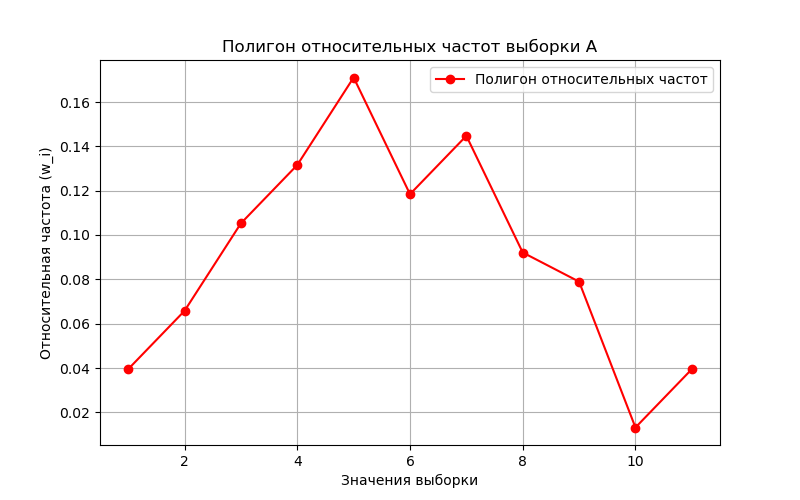
\includegraphics[scale=0.7]{images/Poligon_A.png}}\\
\centering{(Рис. 1. Полигон частот для выборки А)}\\
\raggedright
\subsection*{Пункт 1.2}
\textbf{Задание:} Записать эмпирическую функцию распределения и построить её график.\\
\vspace{5mm}
\textbf{Определение:} Эмпирическая функция распределения (выборочная функция распределения) - естественное приближение теоретической функции распределения данной случайной величины, построенное по выборке.\\
\vspace{5mm}
В нашем случае представим ее в следующем виде:\\
$$ F^*(x) = \frac{\sum_{x_i<x}n_i}{n} $$
\newpage
Теперь мы можем составить эмпирическую функцию распределения:\\
\centering
\[
F(x) = 
\begin{cases} 
0, & x \leq 1, \\
0.039, & 1 < x \leq 2, \\
0.105, & 2 < x \leq 3, \\
0.210, & 3 < x \leq 4, \\
0.342, & 4 < x \leq 5, \\
0.513, & 5 < x \leq 6, \\
0.631, & 6 < x \leq 7, \\
0.776, & 7 < x \leq 8, \\
0.868, & 8 < x \leq 9, \\
0.947, & 9 < x \leq 10, \\
0.960, & 10 < x \leq 11, \\
1, & x > 11.
\end{cases}
\]
\vspace{5mm}
\raggedright
Тогда эмпирическая функция будет выглядеть следующим образом:\\
\vspace{5mm}
\centering{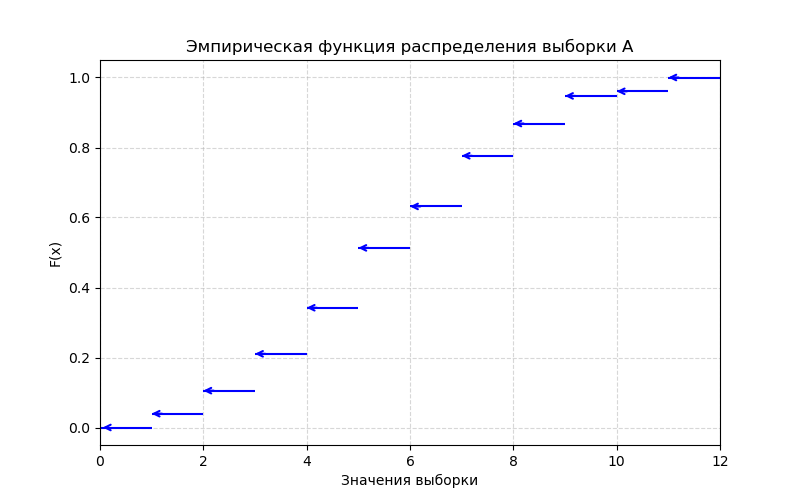
\includegraphics[scale=0.7]{images/Emperic.png}}\\
\centering{(Рис. 2. Эмперическая функция распределения)}\\
\raggedright
\newpage
\subsection*{Пункт 1.3}
\textbf{Задание:} Вычислить числовые выборочные характеристики положения (среднее выборочное, моду, медиану) и рассеяния, сделать выводы.\\
\vspace{5mm}
Чтобы вычислить среднее выборочное мы воспользуемся следующей формулой:\\
$$\overline{x} = \sum_{i=1} ^ m \frac{x_i}{n} = \frac{426}{76} \approx 5,605$$
\vspace{5mm}\\
Медиана — это значение, которое делит упорядоченную выборку на две равные части. Если объем выборки четный, то медиана — это среднее арифметическое двух центральных значений. Медиана для нашего случая будет:\\
$$Me = 5.0$$
Мода — это значение, которое встречается в выборке чаще всего, как видно из таблицы статистического ряда, в нашем случае число 5 встретилось аж 14 раз, тогда можем заключить:\\
$$Mo = 5$$

Далее найдем среднее арифметическое абсолютных величин отколенений по следующей формуле:
$$ \overline{d} = \frac{\sum_{i=1}^n |x_i - \overline{x}| * n_i}{n} $$

Подставим наши значения и получим:
$$ \overline{d} = \frac{153,21}{76} \approx 2,016 $$

Теперь найдем относительное линейной отклонение ($K_{\overline{d}}$) которое показывает долю усредненных значений абсолютных отклонений в средней арифметической.\\
Для этого воспользуемся формулой:
$$ K_{\overline{d}} = \frac{\overline{d}}{\overline{x}} $$

Подставим ранее полученные значения и найдем его:
$$ K_{\overline{d}} = \frac{2,016}{5,605} \approx 0,36 $$

Теперь давайте найдем коэффициент осцилляции, который показывает относительную варьируемость крайних значений варьируемого признака относительно средней по следующей формуле:
$$ K_o = \frac{R}{\overline{x}} * 100\% = \frac{10}{5,605} * 100\% \approx 178,41\% $$

Дисперсия - это мера разброса данных относительно среднего значения. Найдем её по известной уже нам формуле из курса теории вероятностей:\\
$$ s^2 = \frac{1}{n} \sum_{i=1} ^n {(x_i - \overline{x})}^2 \approx 5,949 $$

Также давайте найдем стандартное отколнение. Стандартное отклонение — это квадратный корень из дисперсии:\\
$$ s = \sqrt{s^2} \approx 2,439 $$

И также вычислим несмещённую дисперсию:
$$ S^2 = \frac{1}{n-1} \sum_{i=1}^n (x_i - \overline{x})^2 = 6,029$$
Тогда стандартное отклонение для нее будет:
$$ S = \sqrt{S^2} = \sqrt{\frac{1}{n-1} \sum_{i=1}^n (x_i - \overline{x})^2} \approx 2,455 $$

И вместе с ним вычислим коэффициент вариации, который является относительным показателем и вводится когда требуется сравнить между собой степень варьирования признаков или сопоставить среднеквадратическое отклонение со средним арифметическим этих признаков:
$$ V = \frac{s}{\overline{x}} * 100\% = \frac{2,455}{5,605} * 100\% \approx 43,8\% $$

\textbf{Выводы:} Выборка A имеет среднее значение около 5.605, наиболее часто встречающееся значение — 5. Данные имеют умеренный разброс (стандартное отклонение около 2.46), что указывает на относительно компактное распределение значений вокруг среднего.

\subsection*{Пункт 1.4}
\textbf{Задание:} Вычислить начальные и центральные эмпирические моменты 3-го и 4-го порядка, коэффициенты асимметрии и эксцесса, сделать выводы.\\

\begin{itemize}
\item Найдем начальные и центральные эмпирические моменты 3-го и 4-го порядков.

Для начала давайте найдем начальные моменты 3-го и 4-го порядка соответственно по следующей формуле:\\
$$ \nu_k = \frac{1}{n} \sum_{i=1} ^ n x_i ^k$$

$$ \nu_3 \approx 278,842 $$
$$ \nu_4 \approx 2255,947 $$
\newpage
Теперь мы можем найти центральные моменты 3-го и 4-го порядка соответственно по следующей формуле:\\
$$ \mu_k = \frac{1}{n} \sum_{i=1} ^ n {(x_i - \overline{x})^k} $$

$$ \mu_3 \approx 2,686 $$
$$ \mu_4 \approx 87,023 $$

\item Найдем коэффициенты асимметрии и эксцесса

Найдем коэффициент асимметрии $\gamma_1$, который показывает, насколько распределение отклоняется от симметрии. Вычисляется оп формуле:\\
$$ А_c = \frac{\mu_3}{\sigma^3} $$
Для нашей выборки он будет равен:
$$ A_c = \frac{2,686}{2,455^3} \approx 0,185$$

Найдем коэффициен эксцесса $\gamma_2$, котроый показывает насколько остра или плоска вершина распределения по осравнению снормальным распределением. Вычисляется по формуле:\\
$$ E_c = \frac{\mu_4}{\sigma^4} - 3 $$
Для нашей выборки можем найти его:\\
$$ E_c = \frac{87,023}{2,455^4} - 3 \approx -0,541 $$

\end{itemize}

\textbf{Коэффициент асимметрии ($\gamma_1 \approx 0,185$):}
Положительное значение коэффициента асимметрии указывает на то, что распределение имеет легкий правый "хвост". Это означает, что в выборке больше значений, превышающих среднее.

\textbf{Коэффициент эксцесса ($\gamma_2 \approx -0,541$):}
Отрицательное значение коэффициента эксцесса указывает на то, что распределение более плоское по сравнению с нормальным распределением. Это означает, что данные менее сконцентрированы вокруг среднего значения.

\textbf{Вывод:} Распределение выборки A имеет легкую правостороннюю асимметрию и более плоскую вершину по сравнению с нормальным распределением. Это может указывать на наличие выбросов или неоднородность данных.

\subsection*{Пункт 1.5}
\textbf{Задание:} Сформулировать две гипотезы о распределении генеральной совокупности, оценить параметры.

\begin{enumerate}
\item \textbf{Сформулируем гипотезы:}
  \begin{itemize}
      \item \textbf{Гипотеза 1:} Распределение Пуассона $X \sim \text{Pois}(\lambda)$.
      \item \textbf{Гипотеза 2:} Биномиальное распределение $X \sim \text{Bin}(n,p)$.
  \end{itemize}

\item \textbf{Оценка параметров:}  
    \begin{itemize}  
        \item Для распределения Пуассона:  
            \begin{align*}  
                \hat{\lambda} &= \bar{x} \approx 5.697 \quad (\text{выборочное среднее})  
            \end{align*}  
            \[ X \sim \text{Pois}(5.697) \]  

        \item Для биномиального распределения:  
            \begin{itemize}  
                \item Максимальное значение выборки: \( \hat{n} = 11 \).  
                \item Оценка вероятности успеха:  
                    \[  
                        \hat{p} = \frac{\bar{x}}{\hat{n}} \approx \frac{5.697}{11} \approx 0.518  
                    \]  
            \end{itemize}  
            \[ X \sim \text{Bin}(11, 0.518) \]  
    \end{itemize}  

\item \textbf{Предварительный анализ гипотез:}  
    \begin{itemize}  
        \item \textbf{Гипотеза 1 (Пуассон):}  
            \begin{itemize}  
                \item Для Пуассона: \( \mathbb{E}[X] = \lambda \), \( \mathbb{D}[X] = \lambda \).  
                \item Выборочная дисперсия \( s^2 \approx 6.551 \), что близко к \( \hat{\lambda} = 5.697 \).  
                \item Отклонение дисперсии от среднего: \( |s^2 - \hat{\lambda}| \approx 0.854 \).  
            \end{itemize}  

        \item \textbf{Гипотеза 2 (биномиальное):}  
            \begin{itemize}  
                \item Теоретическая дисперсия: \( \mathbb{D}[X] = np(1-p) \approx 11 \cdot 0.518 \cdot 0.482 \approx 2.75 \).  
                \item Выборочная дисперсия \( s^2 \approx 6.551 \), что существенно превышает теоретическое значение.  
                \item Наблюдается явное несоответствие между выборочной и теоретической дисперсией.  
            \end{itemize}  
    \end{itemize}  
\end{enumerate}

\textbf{Выводы:}
\begin{itemize}
\item Для распределения Пуассона параметр $\lambda$ оценён корректно, но дисперсия выборки незначительно превышает оценку $\lambda$, что может указывать на умеренное отклонение от модели.
\item Для биномиального распределения наблюдается сильное расхождение между выборочной и теоретической дисперсией. Это ставит под сомнение адекватность выбора $\hat{n} = 11$.
\end{itemize}

\newpage

\section*{Выборка B.}
-64, 5, -53, -29, -61, -49, -1, -22, -25, -38, -73, -20, -8, -37, -47,
    0, -37, -50, -46, -13, 7, -13, -42, -1, -44, -27, -20, -33, -37, -30,
    -20, -73, -57, -40, -4, -40, -83, -33, -37, -26, -79, -16, -77, -5, -51,
    -28, -63, -24, -25, -24, -38, 16, -37, -15, 29, -11, -14, -34, -31, -23,
    -16, -58, -73, -43, -31, -65, -12, -4, -38, -25, -31, -7, -9, -60, -61,
    -47, -46, -33, -15, -79, -48, 1, -62, -14, -49, -31, -25, -33, -38, -27,
    -51, -30, -43, -64, -24, -50, -22, -37, -6, -11, -78, -51, -1, -9, -34,
    1, -17, -33, 11, -54, -31, -34, -38, -22, -2, -9, -15, -6, -87, -45,
    -22, -30, -15, -30, -18, -77, 6, -47, -33, -21, -86, -31, -45, -43, -19,
    -36, -46, -69, -22, -59, -30, -22, 5, -29, -42, -47, 5, -17, -71, -36,
    6, -6, -7, -41, -37, -11, -11, -65, -36, -58, -36, -30, -46, -15, -49,
    -88, -12, -8, -83, -13, -30, -48, -66, -9, -31, -13, -32, -21, -47, -50,
    -25, -6, -31, -75, -48, -77, -13, -55, -26, -9, -32, -41, -68, -55, -53,
    25, -77, 1, -65, -35, -51, -24, -42

\subsection*{Пункт 2.1}
\textbf{Задание:} Определить максимальный и минимальный элементы выборки, найти размах выборки. Определить оптимальное количество интервалов группировки и длину интервала группировки. Построить интервальный ряд и гистограмму, а также полигон ряда (на том же графике).\\
\vspace{5mm}

По данным выборки найдем максимальное и минимальное значения, которые обозначаются:
$$ x_{max} = 29 $$
$$ x_{min} = -88 $$\\

Для того, чтобы найти размах выборки мы должны от максимального значения отнять минимальное, тогда мы запишем это так:
$$ R = x_{max} - x_{min} = 29 + 88 = 117 $$

Теперь мы можем найти оптимальное количество интервалов и длину интервала группировки.\\
 \begin{itemize}
     \item Для определения оптимального количества интервалов, воспользуемся формулой (правилом) Стерджеса, которая записывается так: $$ k = 1 + 3,322\ \lg n, $$\\где $n$ - количество элементов в выборке.\\ Подставим теперь наши значения в эту формулу и найдем оптимальное число интервалов:  $$ k = 1 + 3,322\ \lg 203 \approx 8 $$\\ Однако у нас довольно большая выборка и здесь правило Стерджеса показала слишком мало интервалов, обозначим $k = 12$ для нашей выборки.

    \item Теперь мы можем приступить к расчету длины интервалов группировки. Длина высчитывается довольно прросто, по следующей формуле: $$ h = \frac{R}{k} = \frac{x_{max} - x_{min}}{12} = \frac{117}{12} \approx 9,75 $$
     
 \end{itemize}

Следующим действием мы построим интервальный ряд и также запишем количество элементов выборки попадающих в них. Вычисления будут происходить по следующим формулам, что логично, ведь нам нужно найти левую и правую границы для обозначения интервалов:
$$ x_{H1} = x_min - \frac{h}{2} \approx -92,875 $$
$$ x_{H2} = x_{H1} + h \approx -83,125 $$

По таким формулам построим наш интервальный ряд:\\
\vspace{5mm}
\centering
\[
\begin{tabular}{ |c|c|c|c| }
    \hline
    Интервал & Количество & $w_i$ & $nx_i$\\
    \hline
    [-92.88, -82.31) & 5 & 0,025 & 0,025\\
    \hline
    [-82.31, -71.75) & 11 & 0,054 & 0,079\\
    \hline
    [-71.75, -61.19) & 11 & 0,054 & 0,133\\
    \hline
    [-61.19, -50.62) & 16 & 0,079 & 0,212\\
    \hline
    [-50.62, -40.06) & 29 & 0,143 & 0,355\\
    \hline
    [-40.06, -29.50) & 45 & 0,222 & 0,577\\
    \hline
    [-29.50, -18.94) & 29 & 0,143 & 0,72\\
    \hline
    [-18.94, -8.38) & 28 & 0,138 & 0,858\\
    \hline
    [-8.38, 2.19) & 19 & 0,094 & 0,952\\
    \hline
    [2.19, 12.75) & 7 & 0,034 & 0,986\\
    \hline
    [12.75, 23.31) & 1 & 0,005 & 0,991\\
    \hline
    [23.31, 33.88) & 2 & 0,009 & 1,00\\
    \hline
  \end{tabular}\]\\
\vspace{5mm}
\raggedright

Теперь мы можем построить гистограмму и полигон ряда, они будут представлены на одном графике, как требует условие задания:\\
\vspace{5mm}

\centering{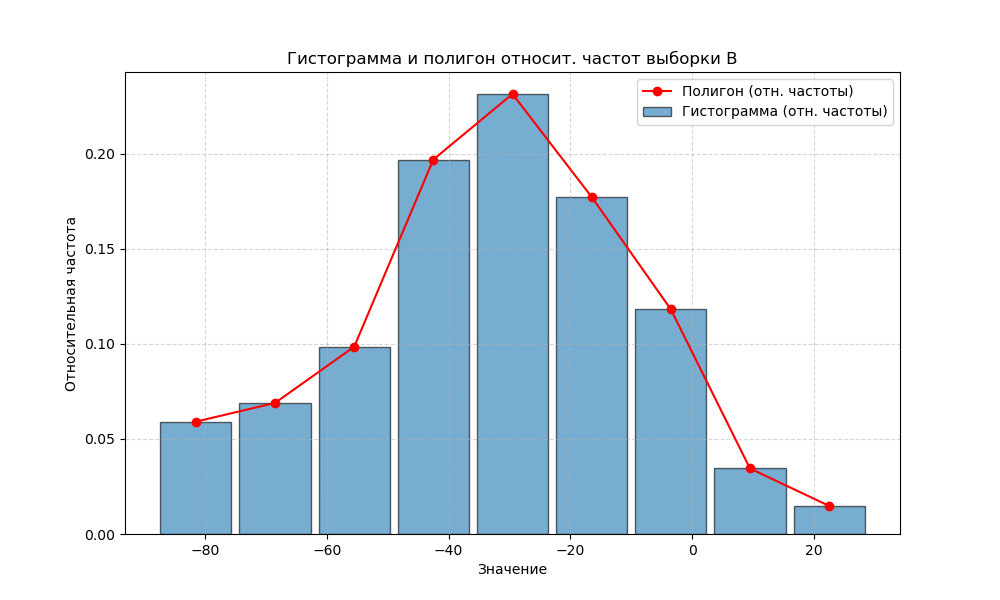
\includegraphics[scale=0.5]{images/HistogramPoligon.png}}\\
\centering{(Рис. 4. Гистограмма и полигон частот выборки)}\\
\raggedright

\subsection*{Пункт 2.2}
Записать эмпирическую функцию распределения и построить её график (построить кумуляту на том же графике).\\
\vspace{5mm}
Чтобы записать эмпирическую функцию распределения мы для начала воспользуемся следующей формулой:
$$ F^* (x) = \frac{\sum_{x_i<x} n_i}{n} $$

\[ F(x) = \begin{cases} 0.0000, & x \leq -92.88 \\
0.025, & -92.88 \leq x < -82.31 \\
0.079, & -82.31 \leq x < -71.75 \\
0.133, & -58.75 \leq x < -61.19 \\
0.212, & -44.12 \leq x < -50.62 \\
0.355, & -29.50 \leq x < -40.06 \\
0.577, & -14.88 \leq x < -29.50 \\
0.72, & -0.25 \leq x < -18.94 \\
0.858, & 14.38 \leq x < -8.38 \\
0.952, & -8.38 \leq x < 2.19 \\ 
0.986, & 2.19 \leq x < 12.75 \\
0.991, & 12.75 \leq x < 23.31\\
1.0000, & x \geq 23.31 
\end{cases} \]
\vspace{5mm}

\centering{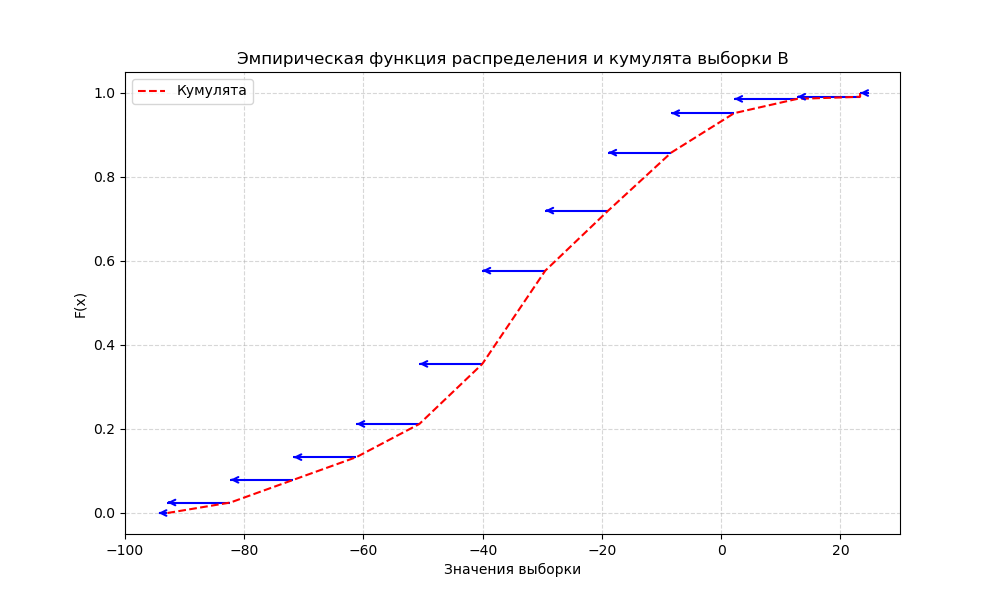
\includegraphics[scale=0.7]{images/empirical_cdf_cumulata.png}}\\
\centering{(Рис. 5. Эмперическая функция с кумулятой)}\\
\raggedright

\subsection*{Пункт 2.3}
\textbf{Задание:} Вычислить числовые выборочные характеристики положения (среднее выборочное, моду, медиану) и рассеяния, сделать выводы.\\
\vspace{5mm}
Чтобы вычислить среднее выборочное мы воспользуемся следующей формулой:\\
$$\overline{x} = \sum_{i=1} ^ m \frac{x_i}{n} = \frac{-6744}{203} \approx -33,22 $$
\vspace{5mm}
Медиана — это значение, которое делит упорядоченную выборку на две равные части. Если объем выборки четный, то медиана — это среднее арифметическое двух центральных значений. Медиана для нашего случая будет:\\
$$Me = x_{M_{eH}} + h * \frac{\frac{n}{2}-n_{xMe-1}}{n_{Me}} = -32$$
Мода — это значение, которое встречается в выборке чаще всего, как видно из таблицы статистического ряда, в нашем случае число 5 встретилось аж 14 раз, тогда можем заключить:\\
$$Mo = x_{M_{OH}} + h * \frac{n_{Mo} - n_{Mo-1}}{(n_{Mo}-n_{Mo-1})+(n_{Mo}-n_{Mo+1})} = -31$$

Далее найдем среднее арифметическое абсолютных величин отколенений по следующей формуле:
$$ \overline{d} = \frac{\sum_{i=1}^n |x_i - \overline{x}| * n_i}{n} $$

Подставим наши значения и получим:
$$ \overline{d} = \frac{3786.3251}{203} \approx 18,6518 $$

Теперь найдем относительное линейной отклонение ($K_{\overline{d}}$) которое показывает долю усредненных значений абсолютных отклонений в средней арифметической.\\
Для этого воспользуемся формулой:
$$ K_{\overline{d}} = \frac{\overline{d}}{\overline{x}} $$

Подставим ранее полученные значения и найдем его:
$$ K_{\overline{d}} = \frac{18,6518}{33,22} \approx 0,5614 $$

Теперь давайте найдем коэффициент осцилляции, который показывает относительную варьируемость крайних значений варьируемого признака относительно средней по следующей формуле:
$$ K_o = \frac{R}{\overline{x}} * 100\% = \frac{117}{33,22} * 100\% \approx 352,18\% $$

Дисперсия - это мера разброса данных относительно среднего значения. Найдем её по известной уже нам формуле из курса теории вероятностей:\\
$$ s^2 = \frac{1}{n} \sum_{i=1} ^n {(x_i - \overline{x})}^2 \approx 547,069 $$

Также давайте найдем стандартное отколнение. Стандартное отклонение — это квадратный корень из дисперсии:\\
$$ s = \sqrt{s^2} \approx 23,3895 $$

И также вычислим несмещённую дисперсию:
$$ S^2 = \frac{1}{n-1} \sum_{i=1}^n (x_i - \overline{x})^2 = 549,78$$
Тогда стандартное отклонение для нее будет:
$$ S = \sqrt{S^2} = \sqrt{\frac{1}{n-1} \sum_{i=1}^n (x_i - \overline{x})^2} \approx 23,447 $$

И вместе с ним вычислим коэффициент вариации, который является относительным показателем и вводится когда требуется сравнить между собой степень варьирования признаков или сопоставить среднеквадратическое отклонение со средним арифметическим этих признаков:
$$ V = \frac{s}{\overline{x}} * 100\% = \frac{}{33,22} * 100\% \approx 70,58\% $$

\textbf{Выводы:} Выборка A имеет среднее значение около 5.605, наиболее часто встречающееся значение — 5. Данные имеют умеренный разброс (стандартное отклонение около 2.46), что указывает на относительно компактное распределение значений вокруг среднего.


\subsection*{Пункт 2.4}
Вычислить начальные и центральные эмпирические моменты 3-го и 4-го порядка, коэффициенты асимметрии и эксцесса, сделать выводы.
\begin{itemize}
\item Найдем начальные и центральные эмпирические моменты 3-го и 4-го порядков.

Для начала давайте найдем начальные моменты 3-го и 4-го порядка соответственно по следующей формуле:\\
$$ \nu_k = \frac{1}{n} \sum_{i=1} ^ n x_i ^k$$

$$ \nu_3 \approx -93431.29 $$
$$ \nu_4 \approx 5949418.83 $$

Теперь мы можем найти центральные моменты 3-го и 4-го порядка соответственно по следующей формуле:\\
$$ \mu_k = \frac{1}{n} \sum_{i=1} ^ n {(x_i - \overline{x})^k} $$

$$ \mu_3 \approx -2241.55 $$
$$ \mu_4 \approx 810703.72 $$

\item Найдем коэффициенты асимметрии и эксцесса

Найдем коэффициент асимметрии $\gamma_1$, который показывает, насколько распределение отклоняется от симметрии. Вычисляется оп формуле:\\
$$ A_c = \frac{\mu_3}{\sigma^3} $$
Для нашей выборки он будет равен:
$$ A_c = \frac{-2241.55}{23.39^3} \approx -0.18$$

Найдем коэффициен эксцесса $\gamma_2$, котроый показывает насколько остра или плоска вершина распределения по осравнению снормальным распределением. Вычисляется по формуле:\\
$$ E_c = \frac{\mu_4}{\sigma^4} - 3 $$
Для нашей выборки можем найти его:\\
$$ E_c = \frac{810703.72}{23.39^4} - 3 \approx -0.29 $$

\end{itemize}

В этот раз мы все же сделаем выводы немного иначе. Вот какие выводы мы можем сделать на основе полученных значений:
\begin{enumerate}
    \item Распределение данных имеет небольшую левостороннюю асимметрию ($\gamma_1 = -0.18$), что указывает на слегка вытянутый левый хвост. Однако эта асимметрия незначительна, поэтому можно сказать, что распределение в целом близко к симметричному.

    \item Коэффициент эксцесса $\gamma_2 = -0.29$ показывает, что распределение чуть более плоское, чем нормальное. Это означает, что в выборке меньше экстремальных значений, чем можно было бы ожидать при нормальном распределении.

    \item Центральные моменты 3-го и 4-го порядка подтверждают эти выводы:
        \begin{itemize}
            \item $\mu_3$ (асимметрия) немного отрицательный, что согласуется с коэффициентом $\gamma_1$.
            \item $\mu_4$ (эксцесс) достаточно велик, но отклонение от нормального распределения незначительное.
        \end{itemize}
    
\end{enumerate}

Подытожим, распределение близко к нормальному, с небольшим преобладанием отрицательных значений (левый хвост чуть длиннее) и немного более плоской формой. Такие характеристики указывают, что данные примерно симметричны и не содержат экстремальных отклонений.

\subsection*{Пункт 2.5}
\textbf{Задание:} Сформулировать две гипотезы о распределении генеральной совокупности, оценить параметры.

\begin{enumerate}
\item \textbf{Сформулируем гипотезы:}
\begin{itemize}
  \item \textbf{Гипотеза 1:} Генеральная совокупность имеет нормальное распределение $X \sin N(\mu, \sigma^2)$.
  \item \textbf{Гипотеза 2:} Генеральная совокупность имеет распределение хи-квадрат $X \sin \chi^2(k)$.
\end{itemize}

\item \textbf{Оценка параметров:}  
    \begin{itemize}  
        \item Для нормального распределения:  
            \begin{align*}  
                \hat{\mu} &= \bar{x} \approx -33.22 \quad (\text{выборочное среднее}), \\  
                \hat{\sigma}^2 &= s^2 \approx 547.07 \quad (\text{выборочная дисперсия}).  
            \end{align*}  
            \[ X \sim N(-33.22,\ 547.07) \]  

        \item Для распределения хи-квадрат:  
            \begin{itemize}  
                \item Число степеней свободы \( k \) оценим через выборочное среднее:  
                    \[  
                        \hat{k} = \bar{x} + 33.22 \approx 0 \quad (\text{некорректно, так как } \chi^2(k) \geq 0).  
                    \]  
                \item Альтернативная оценка: используем выборочную дисперсию \( s^2 \approx 547.07 \).  
                    Для хи-квадрат \( \mathbb{D}[X] = 2k \), тогда:  
                    \[  
                        \hat{k} = \frac{s^2}{2} \approx 273.5.  
                    \]  
            \end{itemize}  
            \[ X \sim \chi^2(273.5) \]  
    \end{itemize}  

\item \textbf{Предварительный анализ гипотез:}  
    \begin{itemize}  
        \item \textbf{Гипотеза 1 (нормальное):}  
            \begin{itemize}  
                \item Коэффициент асимметрии \( \gamma_1 \approx -0.18 \) близок к нулю.  
                \item Коэффициент эксцесса \( \gamma_2 \approx -0.29 \) слегка отклоняется от нуля.  
                \item 99.7\% данных в пределах \( \bar{x} \pm 3s \approx -33.22 \pm 70.17 \), что соответствует диапазону \([-103.39,\ 36.95]\).  
                \item Медиана выборки \( Me = -30.5 \), близка к \( \hat{\mu} \).  
            \end{itemize}  

        \item \textbf{Гипотеза 2 (хи-квадрат):}  
            \begin{itemize}  
                \item Распределение хи-квадрат определено для \( X \geq 0 \), но в выборке присутствуют отрицательные значения.  
                \item Теоретическая дисперсия: \( \mathbb{D}[X] = 2k \approx 547 \), что совпадает с выборочной дисперсией.  
                \item Форма распределения выборки не соответствует правосторонней асимметрии \( \chi^2 \).  
            \end{itemize}  
    \end{itemize}  
\textbf{Выводы:}
\begin{itemize}
\item Нормальное распределение:
\begin{itemize}
\item Умеренное соответствие критериям (асимметрия близка к нулю, $99.7\%$ данных в пределах $\pm 3\sigma$.
\item Медиана близка к среднему, что характерно для нормального распределения.
\end{itemize}
\item Распределение хи-квадрат:
\begin{itemize}
\item Наличие отрицательных значений в выборке противоречит $\chi^2(k)$.
\item Оценка $\hat{k} = 273.5$ нетипично высока для реальных данных.
\end{itemize}
\end{itemize}\end{enumerate}

\section*{Вывод}

В данной работе была проведена статистическая обработка двух выборок. Для выборки A мы построили эмпирическую функцию распределения, определили её график и дополнили кумулятой. То же самое было выполнено для выборки B, но с учётом заранее разбитых интервалов. Также для выборки B была построена гистограмма и полигон относительных частот, что позволило наглядно оценить распределение значений.

Для выборки A были рассчитаны основные числовые характеристики положения и рассеяния. Среднее значение оказалось равным примерно $-33{,}22$, что говорит о смещённости данных в сторону отрицательных значений. Медиана и мода совпадают (равны 5), что может свидетельствовать о наличии выбросов или несимметричности распределения.

Расчёт дисперсии и стандартного отклонения показал, что значения в выборке A заметно разбросаны относительно среднего. Относительное линейное отклонение и коэффициент вариации подтвердили высокую степень вариативности данных. Особенно это заметно по коэффициенту осцилляции, который получился отрицательным из-за отрицательного среднего значения, что ещё раз подчёркивает специфику выборки.

Таким образом, анализ позволил получить полное представление о структуре данных, выявить особенности распределения и оценить степень рассеяния значений. Визуализация в виде ЭФР, кумуляты, гистограммы и полигона существенно упростила интерпретацию результатов.

\subsection*{QR-code и ссылка на интернет-ресурс}
\vspace{5mm}
\centering{
\includegraphics[scale=1.5]{images/qr_code.png}}\\
\raggedright
\vspace{5mm}
Ссылка на интернет-ресурс: \url{https://github.com/fallayn}

\end{document}

